\subsection{Prediction Target: FIMA NFIP Claims}
Our prediction target is derived from the OpenFEMA FIMA NFIP Redacted Claims Dataset v2~\cite{fema_nfip_claims_v2}, which records every NFIP insurance claim filed under the National Flood Insurance Program, including the reported \texttt{dateOfLoss}, redacted location (Census Tract, ZIP code, and nearest $0.1^{\circ}\times 0.1^{\circ}$ grid cell), \texttt{causeOfDamage} category, and paid amounts for building and contents coverage.
%
As we target pluvial claims, we filter the dataset to include only those claims defined as \texttt{causeOfDamage} = \texttt{Accumulation of rainfall or snowmelt}, which serve as the supervisory signal for our prediction task.
%
NFIP data, while the most comprehensive source of insured flood damage in CONUS, is known to have uncertainties and errors in both space and time~\cite{wing_new_2020,petkov_learning_2025,shin_systematic_2022}.
%
To improve learning dynamics and model validation, we apply two correction methods, temporal and spatial, to mitigate these uncertainties.

% \subsubsection{Temporal and Spatial Uncertainty Correction}
% %
% Such data noise pose challenges in effective learning. 
% %
% To improve learning dynamics and model validation, we target two sources of uncertainty in the NFIP claims data: temporal and spatial.
% %
\subsubsection{Temporal Uncertainty Correction}\label{ssec:temporal_correction}
The \texttt{dateOfLoss} field in the NFIP claims data is known to be noisy where reported dates of loss often fail to align with precipitation events in the historical precipitation records.
%
These discrepancies may arise from reporting lags, human error during claim filing, and misclassification of \texttt{causeOfDamage}, where fluvial or coastal damages are mislabeled as pluvial~\cite{shin_systematic_2022}.
%
To mitigate this noise, we apply the following correction to the \texttt{dateOfLoss} field $d$:
\begin{enumerate}[nosep, align=left, leftmargin=*, left=1pt]
    \item Compute the daily maximum hourly accumulated precipitation from NOAA AORC~\cite{fall_analysis_2023} for day $d$ at the location of the claim.
    \item If the daily maximum hourly accumulated precipitation on day $d$ exceeds 10\,mm, accept \texttt{dateOfLoss} as reported.
    \item Otherwise, search the window $d' \in \{d-3, \ldots, d+3\}$ and select the day with the largest daily maximum hourly precipitation. If this maximum exceeds 10\,mm, update \texttt{dateOfLoss} to $d'$.
    \item If no day's daily maximum hourly precipitation in the window exceeds 10\,mm, discard the claim as erroneous.
\end{enumerate}

\noindent
We adopt 10\,mm as a \textit{conservative} threshold for maximum hourly accumulated precipitation, sitting between two reference points. 
%
National Weather Service Flash Flood Guidance (FFG) thresholds are most predictive for most areas when hourly precipitation exceeds \tsim$25.4$\,mm~\cite{james_precipitation_2024}, while the American Meteorological Society's Glossary of Meteorology defines \textit{heavy} precipitation as 7.62\,mm in one hour~\cite{ams_glossary_rain}.
%
% Table~\ref{tab:date_shifts} summarizes the resulting shift distribution. 
With this processing, $81.1\%$ of claims are accepted as reported, $12.9\%$ are shifted within $\pm 3$ days, and $6.0\%$ are discarded.
%
We place the full table of date shifts in the Appendix.

\subsubsection{Spatial Uncertainty Correction}\label{ssec:spatial_correction}
The address-level claims data is not publicly available and the redacted claims data is only identifiable by its Census Tract, Zip Code and the nearest $0.1^{\circ}\times 0.1^{\circ}$ degree cell.
%
% This spatial uncertainty in the exact location is problematic for learning.
To mitigate this spatial uncertainty of the location of the claim, for every claim, we retrieve the intersection of the reported Census Tract, Zip Code, and the $0.1^{\circ}\times 0.1^{\circ}$ cell centered on the reported coordinate, yielding a polygon for each claim.
%
After this spatial uncertainty correction, our median polygon area for each claim is $\sim1.7$km$^2$ with a mean area of $\sim7.7$km$^2$ due to a significant right tail of large rural polygons.


\subsection{Study Region and Period}\label{ssec:study_region}
We segment CONUS into 75$\times$75\,km grid cells and select the top 100 cells by pluvial NFIP damage claim count, yielding a nationally distributed set of the most flood-affected regions rather than blanket coverage of CONUS.
%
These cells span CONUS, while concentrating in the Northeast and Gulf regions of the United States (Fig.~\ref{fig:study_region}), and together account for $\sim$81\% of all pluvial NFIP claims from 2017--2022.
%
Extending to the top 200 cells would raise claim coverage only modestly to $\sim$91\% while roughly doubling the dataset, so we adopt the top 100 as a balance between capturing the large majority of pluvial claims and keeping storage and compute tractable.
%
Within each 75$\times$75\,km grid cell, we further discretize space into a 64$\times$64 raster of \textit{pixels} ($\sim$1.17\,km on a side), which constitute the unit of spatial prediction throughout the remainder of the paper.
%
We restrict our study period to 2017--2022, the longest contiguous interval over which all data sources have full-year coverage.
%
% This window is bounded below by the AlphaEarth Foundation embedding record, which is available annually from 2017, and above by the NWM Retrospective v3.0 dataset, which ends in January 2023.
\begin{figure}[t]
    \centering
    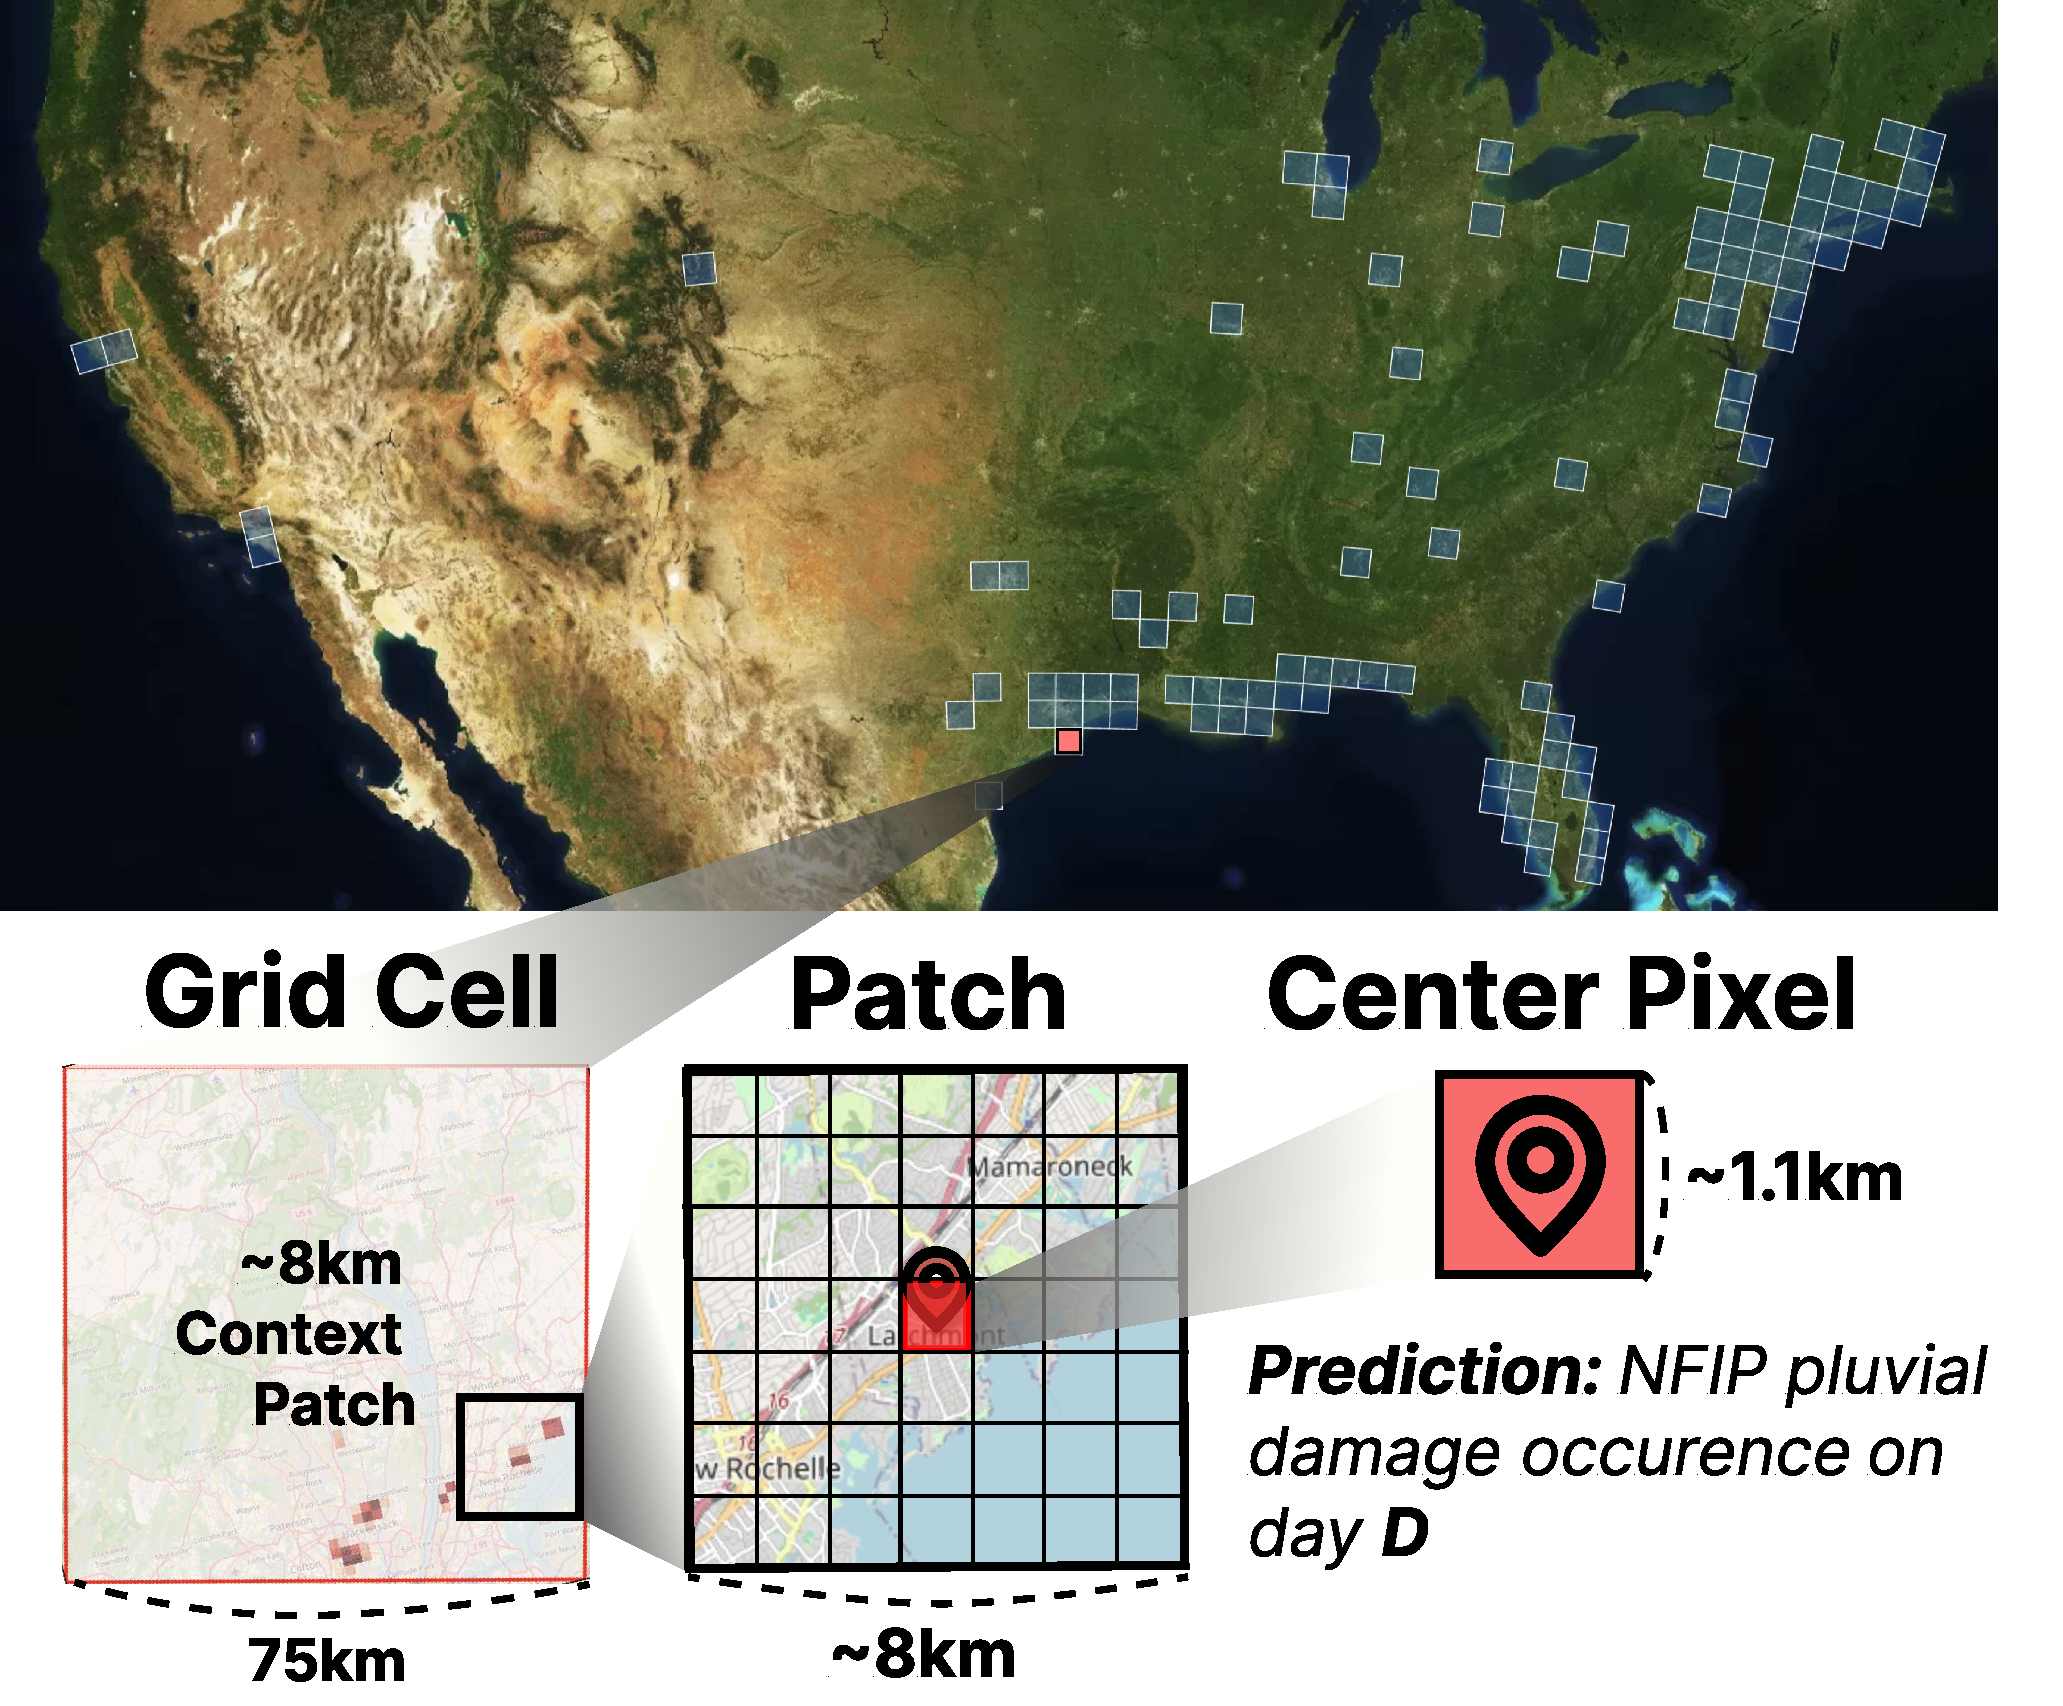
\includegraphics[width=\linewidth]{figs/StudyRegion.pdf}
    \caption{Our study region in blue. We select the Top 100 75$\times$75\,km \emph{grid cells} for NFIP pluvial flood damage claims, accounting for $\sim$81\% of claims from 2017--2022.  After rasterizing NFIP claims (see \S\ref{ssec:temporal_correction},\S\ref{ssec:spatial_correction}), training samples take the form of (\emph{pixel}, day) tuples, and DELUGE takes input a $\sim$8x8km \emph{patch} centered around the \emph{pixel} as spatial context.}
    \label{fig:study_region}
\end{figure}


\subsection{Dataset Construction}\label{ssec:dataset_construction}
The unit of binary prediction is a (pixel, day) tuple over our study region and period, i.e., was there a pluvial NFIP damage claim reported at pixel $p$ on day $d$?
%
First to collect our positive class, we rasterize each claim's spatial-uncertainty polygon (\S\ref{ssec:spatial_correction}) onto the 64$\times$64 grid, labeling every intersecting pixel as positive.
%
To prevent claims with large polygons from dominating the loss, we associate each claim with a confidence score: $c_{claim} = \min(1,\, A_{\text{pix}}/A_{\text{claim}})$ with $A_{\text{pix}} = 1.17^{2}$\,km$^{2}$.
%
To account for pixels with many intersecting claims, we calculate and define our confidence at each pixel $c_{pixel}$ as the complement of the product of each claim's confidence score: $c_{pixel} = 1 - \prod_{i\in\text{claim}}(1 - c_i)$.
%
This operation captures the intuition that multiple claims intersecting a pixel should increase the confidence of a claim for that pixel.
% while also preventing pixels with many intersecting claims from dominating the loss by effectively
% scaling each claim's total contribution toward that of a single-pixel-localized claim.

For the negative class, exhaustively enumerating every pixel-day in our study period would yield a label distribution dominated by trivially negative dry days, further exacerbating class imbalance.
%
We therefore construct the dataset along three data types drawn from two contrastive axes: positives, \textit{spatial} negatives (same-day, different-pixel), and \textit{temporal} negatives (different-day, same-grid).
% \begin{itemize}[noitemsep, topsep=0pt, left=0pt, align=left]    
%
    \textbf{Positives}: \emph{Pixel-days containing at least one NFIP pluvial claim after the temporal and spatial uncertainty corrections described above, along with a confidence score $c$.}
    %
    \textbf{Spatial Negatives}: \emph{Pixel-days without a claim on grid-days that contain at least one claim somewhere within the same 75$\times$75\,km grid cell.}
    %
    \textbf{Temporal Negatives}: \emph{Pixel-days on grid-days where the spatial mean of the 1-hour maximum accumulated precipitation from NOAA AORC exceeds 10\,mm and no NFIP claim was filed anywhere in the grid cell.} 
%
We reuse the 10\,mm threshold from our temporal uncertainty correction (\S\ref{ssec:temporal_correction}) so that meaningful precipitation events are defined consistently across the pipeline.
% \end{itemize}
Despite this undersampling of temporal negatives, the dataset exhibits \emph{significant class imbalance} with a positive rate of \tsim$0.25\%$ across the study region and period.



